% Proposta de figuras para o Cap. II (05/11/2026, pedido do autor). NÃO é parte
% do TG: o autor quer analisar antes de decidir se e onde entram. As três
% figuras são diagramas TikZ desta pasta (fig07, fig08, fig09), compilados pelo
% Makefile. Datas da linha do tempo: cabeçalho do fig07-periodos.tex.
\documentclass[11pt,a4paper]{article}
\usepackage[T1]{fontenc}
\usepackage[brazilian]{babel}
\usepackage{mathptmx}
\usepackage[a4paper,margin=2.4cm]{geometry}
\usepackage{graphicx}
\usepackage[font=small,labelfont=bf]{caption}
\usepackage[most]{tcolorbox}
\usepackage[hidelinks]{hyperref}
\setlength{\parskip}{0.45em}
\setlength{\parindent}{0pt}

\definecolor{cesc}{RGB}{220,50,32}
\definecolor{cmod}{RGB}{0,90,181}
\newtcolorbox{ideia}[1][]{colback=cmod!5, colframe=cmod!70, fonttitle=\bfseries, title={#1}, arc=2pt, boxrule=0.6pt}
\newtcolorbox{cuidado}[1][]{colback=cesc!4, colframe=cesc!70, fonttitle=\bfseries, title={#1}, arc=2pt, boxrule=0.6pt}

\title{Figuras propostas para o Capítulo II\\[2pt]\large períodos, janela de estimação e escolha da configuração}
\author{Material de análise, fora do TG}
\date{5 de novembro de 2026}

\begin{document}
\maketitle

Este relatório reúne três figuras para avaliar antes de qualquer mudança no
texto. A primeira é o Quadro~4 (Períodos de otimização e de teste) redesenhado
como linha do tempo. As outras duas mostram, em desenho, duas ideias que o
Capítulo~II hoje explica só em palavras: a janela deslizante e os três passos da
escolha da configuração. Nada aqui foi colocado no \texttt{tg/}.

\section{Períodos de otimização e de teste}

\begin{figure}[h]
\centering
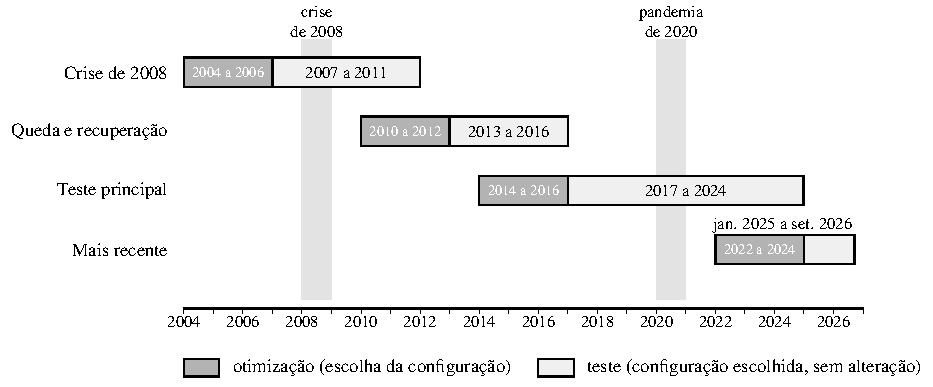
\includegraphics{fig07-periodos.pdf}
\caption{Proposta para substituir o Quadro~4}
\end{figure}

Cada linha é um teste. O trecho escuro são os três anos em que as 312
configurações foram simuladas para escolher uma. O trecho claro, logo ao lado, é o
teste, em que só a escolhida roda. O fato de os dois trechos estarem colados
mostra que o teste começa no pregão seguinte ao fim da otimização. As faixas
cinza marcam 2008 e 2020, os anos que o Capítulo~III analisa à parte.

As configurações fixas, escolhidas em 2010 a 2012, não aparecem: desde
05/11/2026 elas saíram do Capítulo~II e ficaram só como testes adicionais no
Capítulo~III. A figura acompanha o Quadro~4 como ele está agora.

\begin{ideia}[De onde vêm as datas]
As datas das otimizações e dos testes de 2007 a 2011, 2013 a 2016 e 2025 a 2026
vêm da tabela do \texttt{dados/resultados/refeito\_2026-10-05/PROTOCOLO.md}. As de
2017 a 2024 vêm da primeira e da última linha da curva \texttt{curva\_R6\_GS.csv}. A posição de cada
barra é calculada a partir da data, no próprio desenho.
\end{ideia}

\begin{cuidado}[O que se perde em relação ao quadro]
A terceira coluna do quadro (característica do período) virou o rótulo de cada
linha. A faixa de 2020 mostra a pandemia, mas o detalhe ``o mais longo'', do
teste principal, não cabe no rótulo. Se ele for importante, precisa ir para uma
frase do texto.
\end{cuidado}

\clearpage
\section{Janela deslizante de estimação}

\begin{figure}[h]
\centering
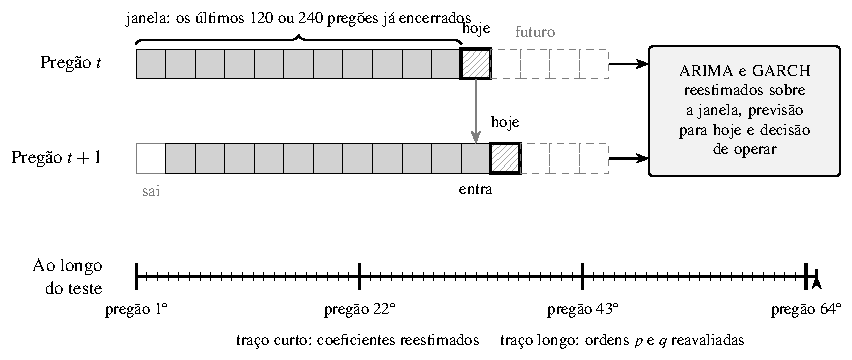
\includegraphics{fig08-janela.pdf}
\caption{Proposta para a seção 2.4.4, Janela de estimação}
\end{figure}

As duas fileiras são dois dias seguidos. No pregão $t$, os modelos são estimados
sobre a janela (cinza) e preveem o pregão de hoje (hachurado). No dia seguinte, o
pregão mais antigo sai, o de ontem, já encerrado, entra, e tudo é estimado de novo.
A faixa de baixo mostra o teste inteiro: os coeficientes mudam todo dia (traço
curto) e as ordens $p$ e $q$ são reavaliadas a cada 21 pregões (traço longo). O
desenho tem menos quadradinhos do que os 120 ou 240 pregões reais. No TG ele
precisaria de uma nota dizendo que é ilustrativo.

\section{Passos da escolha da configuração}

\begin{figure}[h]
\centering
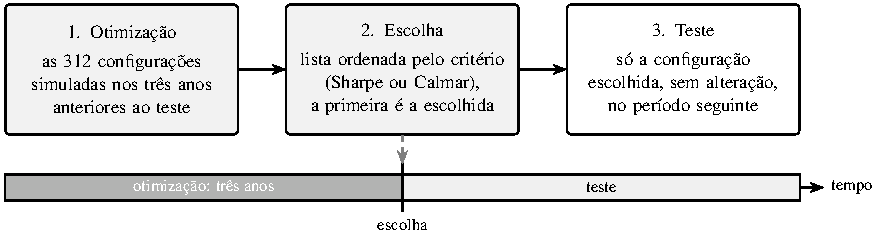
\includegraphics{fig09-escolha.pdf}
\caption{Proposta para a seção Escolha da configuração}
\end{figure}

São os três passos que o texto descreve no parágrafo do teste avançado. A régua
de baixo liga os passos ao tempo: a otimização olha para trás, a escolha acontece
na fronteira, e o teste usa só o que vem depois. É a mesma ideia da linha do tempo
da seção~1, vista para um único teste.

\section{O que mudaria no TG se as três entrassem}

\begin{cuidado}[A lista de ilustrações muda]
Com o Quadro~4 virando figura, o TG fica com 4 quadros. O Manual (4.1.1.10) só
permite lista própria para um tipo que tenha 5 itens ou mais. Por isso as listas
de figuras, de quadros e de gráficos teriam de voltar a ser uma lista única, a
``LISTA DE ILUSTRAÇÕES''. O Quadro~5 (forma de uso do GARCH) passaria a ser o
Quadro~4.
\end{cuidado}

Cada figura também precisaria ser citada no texto (norma). Bastam três frases
curtas de remissão, uma em cada seção. Outro caminho é entrar só com uma ou duas
figuras. Por exemplo, a linha do tempo pode entrar \emph{ao lado} do Quadro~4 em
vez de substituí-lo: assim os quadros continuam 5 e as listas não mudam.
\end{document}
